\documentclass[tikz,border=10pt]{standalone}
\usepackage{tikz}

\definecolor{garnet}{HTML}{73000A}
\definecolor{atlantic}{HTML}{466A9F}
\definecolor{congaree}{HTML}{1F414D}
\definecolor{warmgrey}{HTML}{676156}
\definecolor{horseshoe}{HTML}{65780B}
\definecolor{rose}{HTML}{CC2E40}
\definecolor{honeycomb}{HTML}{A49137}
\definecolor{bk70}{HTML}{5C5C5C}
\definecolor{bk30}{HTML}{C7C7C7}

\begin{document}

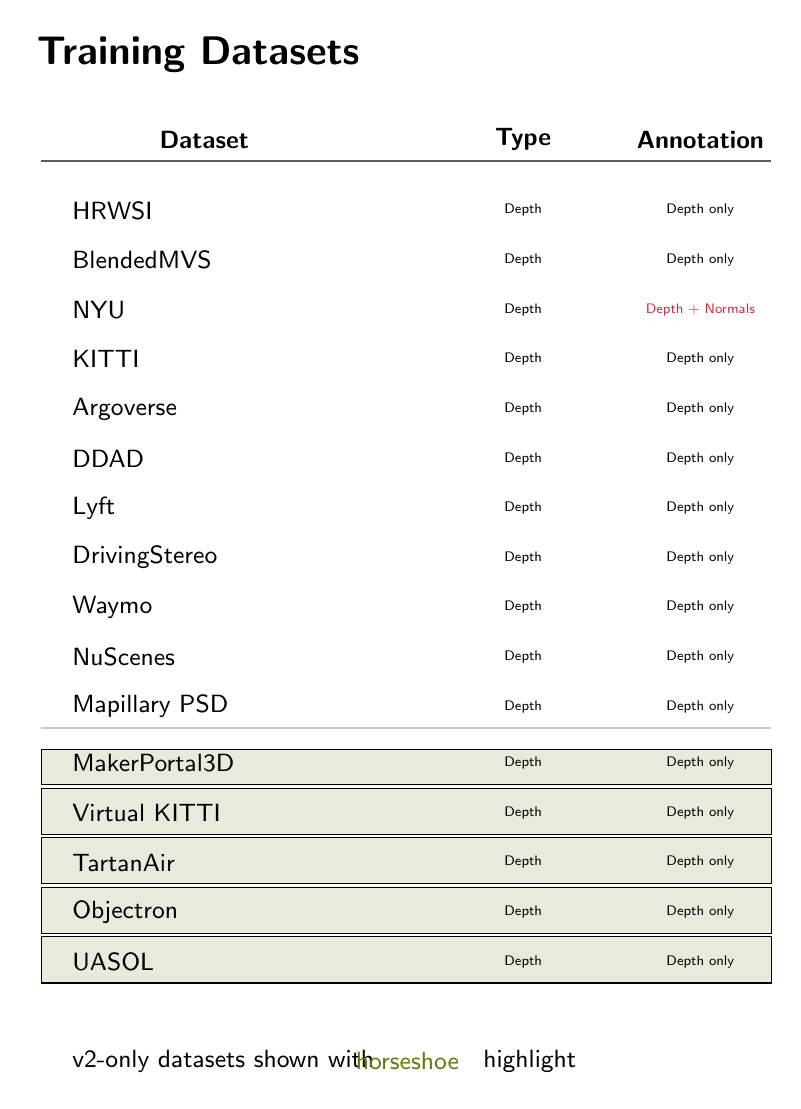
\begin{tikzpicture}[x=0.9cm, y=0.9cm]

% Title
\node[anchor=west, font=\sffamily\bfseries\Large] at (0, 15) {Training Datasets};

% Column headers
\node[anchor=center, font=\sffamily\small\bfseries] at (2.5, 13.8) {Dataset};
\node[anchor=center, font=\sffamily\small\bfseries] at (7, 13.8) {Type};
\node[anchor=center, font=\sffamily\small\bfseries] at (9.5, 13.8) {Annotation};

% Separator line
\draw[line width=0.8pt, color=bk70] (0.2, 13.5) -- (10.5, 13.5);

% v1 datasets (rows 1-11)
\node[anchor=west, font=\sffamily\small] at (0.5, 12.8) {HRWSI};
\node[anchor=center, font=\sffamily\tiny] at (7, 12.8) {Depth};
\node[anchor=center, font=\sffamily\tiny] at (9.5, 12.8) {Depth only};

\node[anchor=west, font=\sffamily\small] at (0.5, 12.1) {BlendedMVS};
\node[anchor=center, font=\sffamily\tiny] at (7, 12.1) {Depth};
\node[anchor=center, font=\sffamily\tiny] at (9.5, 12.1) {Depth only};

\node[anchor=west, font=\sffamily\small] at (0.5, 11.4) {NYU};
\node[anchor=center, font=\sffamily\tiny] at (7, 11.4) {Depth};
\node[anchor=center, font=\sffamily\tiny, color=rose] at (9.5, 11.4) {Depth + Normals};

\node[anchor=west, font=\sffamily\small] at (0.5, 10.7) {KITTI};
\node[anchor=center, font=\sffamily\tiny] at (7, 10.7) {Depth};
\node[anchor=center, font=\sffamily\tiny] at (9.5, 10.7) {Depth only};

\node[anchor=west, font=\sffamily\small] at (0.5, 10) {Argoverse};
\node[anchor=center, font=\sffamily\tiny] at (7, 10) {Depth};
\node[anchor=center, font=\sffamily\tiny] at (9.5, 10) {Depth only};

\node[anchor=west, font=\sffamily\small] at (0.5, 9.3) {DDAD};
\node[anchor=center, font=\sffamily\tiny] at (7, 9.3) {Depth};
\node[anchor=center, font=\sffamily\tiny] at (9.5, 9.3) {Depth only};

\node[anchor=west, font=\sffamily\small] at (0.5, 8.6) {Lyft};
\node[anchor=center, font=\sffamily\tiny] at (7, 8.6) {Depth};
\node[anchor=center, font=\sffamily\tiny] at (9.5, 8.6) {Depth only};

\node[anchor=west, font=\sffamily\small] at (0.5, 7.9) {DrivingStereo};
\node[anchor=center, font=\sffamily\tiny] at (7, 7.9) {Depth};
\node[anchor=center, font=\sffamily\tiny] at (9.5, 7.9) {Depth only};

\node[anchor=west, font=\sffamily\small] at (0.5, 7.2) {Waymo};
\node[anchor=center, font=\sffamily\tiny] at (7, 7.2) {Depth};
\node[anchor=center, font=\sffamily\tiny] at (9.5, 7.2) {Depth only};

\node[anchor=west, font=\sffamily\small] at (0.5, 6.5) {NuScenes};
\node[anchor=center, font=\sffamily\tiny] at (7, 6.5) {Depth};
\node[anchor=center, font=\sffamily\tiny] at (9.5, 6.5) {Depth only};

\node[anchor=west, font=\sffamily\small] at (0.5, 5.8) {Mapillary PSD};
\node[anchor=center, font=\sffamily\tiny] at (7, 5.8) {Depth};
\node[anchor=center, font=\sffamily\tiny] at (9.5, 5.8) {Depth only};

% Separator line before v2 additions
\draw[line width=0.8pt, color=bk30] (0.2, 5.5) -- (10.5, 5.5);

% v2 additional datasets (rows 12-16, highlighted)
\draw[fill=horseshoe, fill opacity=0.15] (0.2, 4.7) rectangle (10.5, 5.2);
\node[anchor=west, font=\sffamily\small] at (0.5, 5) {MakerPortal3D};
\node[anchor=center, font=\sffamily\tiny] at (7, 5) {Depth};
\node[anchor=center, font=\sffamily\tiny] at (9.5, 5) {Depth only};

\draw[fill=horseshoe, fill opacity=0.15] (0.2, 4) rectangle (10.5, 4.65);
\node[anchor=west, font=\sffamily\small] at (0.5, 4.3) {Virtual KITTI};
\node[anchor=center, font=\sffamily\tiny] at (7, 4.3) {Depth};
\node[anchor=center, font=\sffamily\tiny] at (9.5, 4.3) {Depth only};

\draw[fill=horseshoe, fill opacity=0.15] (0.2, 3.3) rectangle (10.5, 3.95);
\node[anchor=west, font=\sffamily\small] at (0.5, 3.6) {TartanAir};
\node[anchor=center, font=\sffamily\tiny] at (7, 3.6) {Depth};
\node[anchor=center, font=\sffamily\tiny] at (9.5, 3.6) {Depth only};

\draw[fill=horseshoe, fill opacity=0.15] (0.2, 2.6) rectangle (10.5, 3.25);
\node[anchor=west, font=\sffamily\small] at (0.5, 2.9) {Objectron};
\node[anchor=center, font=\sffamily\tiny] at (7, 2.9) {Depth};
\node[anchor=center, font=\sffamily\tiny] at (9.5, 2.9) {Depth only};

\draw[fill=horseshoe, fill opacity=0.15] (0.2, 1.9) rectangle (10.5, 2.55);
\node[anchor=west, font=\sffamily\small] at (0.5, 2.2) {UASOL};
\node[anchor=center, font=\sffamily\tiny] at (7, 2.2) {Depth};
\node[anchor=center, font=\sffamily\tiny] at (9.5, 2.2) {Depth only};

% Legend
\node[anchor=west, font=\sffamily\small] at (0.5, 0.8) {v2-only datasets shown with};
\node[anchor=west, font=\sffamily\small, color=horseshoe] at (4.5, 0.8) {horseshoe};
\node[anchor=west, font=\sffamily\small] at (6.3, 0.8) {highlight};

\end{tikzpicture}

\end{document}
